\documentclass[xcolor=dvipsnames]{beamer}
%\documentclass[handout,xcolor=dvipsnames,pdftex,hyperref={colorlinks=false}]{beamer}

%\usetheme{Boadilla}
\usepackage{appendixnumberbeamer}
\usepackage{amssymb}
\usepackage{amsmath}
\usepackage{subfigure}
\usepackage{hyperref}
\usepackage{url}
\usepackage[english]{babel}
\usepackage{natbib}
\newtheorem{assumption}{Assumption}
\usepackage{helvet}
\usepackage{xcolor}
\usepackage{colortbl}
\usepackage{tikz}
\usepackage{booktabs}
\newcommand{\indep}{{\bot\negthickspace\negthickspace\bot}}

\usepackage{bm}
\newcommand\X{{\bm X}}
%\useoutertheme{infolines}


\usetheme{Warsaw}  % Jens' previous
\usepackage{helvet}
\definecolor{someblue}{rgb}{0,.1,0.8}

% == New Commands
% = For general typesetting
\newcommand\spacingset[1]{\renewcommand{\baselinestretch}{#1}\small\normalsize}
\renewcommand\r{\right}
\renewcommand\l{\left}

\newcommand\makegaps{\addtolength{\itemsep}{.25\baselineskip}}
\newcommand\makebiggaps{\addtolength{\itemsep}{.5\baselineskip}}
\newcommand\smallunskip{\vspace{-.25\baselineskip}}
\newcommand\medunskip{\vspace{-.5\baselineskip}}
\newcommand\bigunskip{\vspace{-\baselineskip}}


\newcommand{\VerbBar}{|}
\newcommand{\VERB}{\Verb[commandchars=\\\{\}]}
% Add ',fontsize=\small' for more characters per line
\newcommand{\KeywordTok}[1]{\textcolor[rgb]{0.00,0.44,0.13}{\textbf{{#1}}}}
\newcommand{\DataTypeTok}[1]{\textcolor[rgb]{0.56,0.13,0.00}{{#1}}}
\newcommand{\DecValTok}[1]{\textcolor[rgb]{0.25,0.63,0.44}{{#1}}}
\newcommand{\BaseNTok}[1]{\textcolor[rgb]{0.25,0.63,0.44}{{#1}}}
\newcommand{\FloatTok}[1]{\textcolor[rgb]{0.25,0.63,0.44}{{#1}}}
\newcommand{\CharTok}[1]{\textcolor[rgb]{0.25,0.44,0.63}{{#1}}}
\newcommand{\StringTok}[1]{\textcolor[rgb]{0.25,0.44,0.63}{{#1}}}
\newcommand{\CommentTok}[1]{\textcolor[rgb]{0.38,0.63,0.69}{\textit{{#1}}}}
\newcommand{\OtherTok}[1]{\textcolor[rgb]{0.00,0.44,0.13}{{#1}}}
\newcommand{\AlertTok}[1]{\textcolor[rgb]{1.00,0.00,0.00}{\textbf{{#1}}}}
\newcommand{\FunctionTok}[1]{\textcolor[rgb]{0.02,0.16,0.49}{{#1}}}
\newcommand{\RegionMarkerTok}[1]{{#1}}
\newcommand{\ErrorTok}[1]{\textcolor[rgb]{1.00,0.00,0.00}{\textbf{{#1}}}}
\newcommand{\NormalTok}[1]{{#1}}
\newcommand{\W}{\mathbf{W}}
\newcommand\R{{\bm R}}

\DeclareMathOperator*\plim{plim}
\DeclareMathOperator\rank{rank}
\DeclareMathOperator{\sgn}{sgn}

\DeclareMathOperator{\var}{var}
\DeclareMathOperator{\cov}{cov}
\DeclareMathOperator{\cor}{cor}
\DeclareMathOperator{\sd}{sd}
\DeclareMathOperator{\se}{se}
\DeclareMathOperator{\df}{df}
\DeclareMathOperator{\rv}{RV}
\DeclareMathOperator{\xrv}{XRV}
\DeclareMathOperator{\iv}{IV}
\DeclareMathOperator{\rf}{RF}
\DeclareMathOperator{\fs}{FS}
\DeclareMathOperator{\ar}{AR}
\DeclareMathOperator{\bias}{bias}
\DeclareMathOperator{\BF}{BF}
\DeclareMathOperator{\SeF}{SeF}

\def\independenT#1#2{\mathrel{\rlap{$#1#2$}\mkern2mu{#1#2}}}



\title[]{Sensitivity, especially Omitted Variable Bias}
\subtitle[ ]{Stat 256, Spring 2026}
\author[Hazlett]{Chad Hazlett }
\institute[UCLA]{UCLA\\[1ex]
  \texttt{chazlett@ucla.edu}
}
\date{}

\definecolor{dgreen}{rgb}{0,.6,0.8}
\useoutertheme{infolines}

\begin{document}

\begin{frame}
  \titlepage
\end{frame}

\subject{Talks}
\AtBeginSection[]
{
  \begin{frame}<beamer>
    \frametitle{Outline}
    \tableofcontents[currentsection]
  \end{frame}
}


%======================================================================
\section{Motivation}
%======================================================================

\begin{frame}{Why sensitivity now}
\small
\onslide<1-> So far the workflow has been: pick an ID strategy (e.g.\ CI/SOO), defend the assumptions, estimate well.\\
\bigskip
\onslide<2->  ``Defend the assumptions'' is the fragile one!\\
\bigskip
\onslide<3-> \textbf{Sensitivity analysis}: Don't defend ``confounding=0'', ask ``How strong would confounding have to be to change my research conclusion?'' \\
\bigskip
\begin{itemize}
\item<4-> Warning I will repeat: this is NOT ``how much confounding is there''
\end{itemize}
\bigskip
\onslide<5-> Old idea. Cornfield et al.\ (1959) on smoking and lung cancer:\\
\footnotesize
\begin{quote}
\dots an unobserved confounder \dots would need to lead to a nine-fold increase in the odds of smoking to explain away the association \dots and it was asserted that such a strong unobserved confounder was very unlikely to exist.
\end{quote}
\end{frame}


\begin{frame}{Effects of violence on attitudes: angry or weary?}
\small
\onslide<1-> Among Darfurian refugees in eastern Chad, did exposure to violence on average make people more willing to make concessions to achieve peace (``weary''), or more desiring of retribution (``angry'')?\\
\medskip
\onslide<2-> \textcolor{Blue}{Central ID claim:} targeting of violence in 2003--2004 was based only on village and gender, otherwise highly indiscriminate. \textit{Being directly harmed is ``as-if random within village$\times$gender strata.''}\\
\medskip
\begin{itemize}
\item<3-> Aerial bombing was extremely crude
\item<4-> \textit{Janjaweed} militia attacks targeted on visible characteristics only (notably $\mathit{female}$)
\item<5-> Purpose was to clear population, not target rebels
\end{itemize}
\medskip
\onslide<6-> \textcolor{Blue}{Strategy:} SOO/CI conditioning on village and gender.
\end{frame}


\begin{frame}{Darfur: estimate, and the worry}
\small
\onslide<1-> \textcolor{Blue}{Setup}: outcome \textit{PeaceIndex} (0--1); treatment \textit{DirectHarm} (0/1).\\
\smallskip
\onslide<2->
\[
\mathit{PeaceIndex}_i = \alpha\,\mathit{DirectHarm}_i + \beta^\top \mathit{Village}_i + \phi\, \mathit{female}_i + \epsilon_i.
\]\\
\onslide<3-> Those directly harmed are on average \textcolor{Blue}{9.7 percentage points} more pro-peace (SE $= 2.3$).\\
\medskip
\onslide<4-> \textbf{But what if CI is ``a little'' wrong?}\\
\medskip
\onslide<5-> Questions we'd like sensitivity to help with:\\
\begin{enumerate}
\item<6-> If somebody names a confounder I don't have, how strong would it have to be to overturn the result?
\item<7-> What about \textit{multiple} confounders, possibly acting non-linearly?
\item<8-> How can we report robustness compactly?
\item<9-> How can we make informed guesses about plausible confounding?
\end{enumerate}
\end{frame}


\begin{frame}{A landscape, and our choice}
\onslide<1-> Several families of sensitivity analysis exist:
\small
\begin{itemize}
\item<2-> \textbf{Matched-pair $\Gamma$ bounds} (Rosenbaum 2002): a single odds-of-treatment parameter for matched designs.
\smallskip
\item<3-> \textbf{Parametric} (Imbens 2003; Carnegie--Dorie--Hill 2016): fully specify a model for $(D, Y, U)$, sweep over parameters.
\smallskip
\item<4-> \textbf{Partial identification} (Manski 1990; e.g.\ monotonicity bounds): assume less, get ranges.
\smallskip
\item<5-> \textbf{OVB-based} (Frank 2000; Hosman--Hansen--Holland 2010; \textbf{Cinelli \& Hazlett 2020}): use omitted-variable bias as the engine.
\end{itemize}
\bigskip
\onslide<6-> We focus on OVB-based: scale-free in $R^2$, handles multiple/non-linear confounders, plugs into the regression workflow we just built.
\end{frame}


%======================================================================
\section{FWL and OVB}
%======================================================================

\begin{frame}{A short detour: Frisch--Waugh--Lovell}
\small
\onslide<1-> Suppose we run OLS of $Y$ on $D$ and $\X$:
\[
Y = \hat{\tau}\,D + \X\hat{\beta} + \hat{\epsilon}.
\]
\onslide<2-> The same $\hat{\tau}$ is given by a three-step recipe:
\begin{enumerate}
\item Regress $Y$ on $\X$, take residuals $Y^{\perp \X}$
\item Regress $D$ on $\X$, take residuals $D^{\perp \X}$
\item Regress $Y^{\perp \X}$ on $D^{\perp \X}$
\end{enumerate}
\onslide<3-> In words: \textit{multivariate OLS reduces to univariate OLS, after partialling out $\X$,}
\medskip
\[
\hat{\tau} \;=\; \frac{\cov(D^{\perp \X},\, Y^{\perp \X})}{\var(D^{\perp \X})}.
\]
\onslide<4-> This is the central tool for everything that follows.
\end{frame}


\begin{frame}{Omitted variable bias: setup}
\small
\onslide<1-> Suppose an investigator wishes to run:\\

\begin{align*}
Y &= \hat{\tau}\, D + \X \hat{\beta} + \hat{\gamma}\, Z + \hat{\epsilon}_{\text{full}}
\end{align*}
\onslide<2-> But $Z$ is unobserved, so they run the \textit{restricted} regression:\\
\begin{align*}
Y &= \hat{\tau}_{\text{res}}\, D + \X \hat{\beta}_{\text{res}} + \hat{\epsilon}_{\text{res}}
\end{align*}
\medskip
\onslide<3-> We ask: \textbf{how would $\hat{\tau}$ change if you could include $Z$?}\\

\medskip

\onslide<4-> Whether the ``full'' regression is wise, or its coefficient is the quantity of interest, is a separate question --- here we just compute the consequence of omission.
\end{frame}


\begin{frame}{OVB via FWL: bias $= \hat{\gamma}\hat{\delta}$}
\small
\onslide<1-> Restating FWL,
\[
\hat{\tau}_{\text{res}} \;=\; \frac{\cov(D^{\perp \X},\, Y^{\perp \X})}{\var(D^{\perp \X})}.
\]
\onslide<2-> Substitute the (true) full model $Y = \hat{\tau} D + \X\hat{\beta} + \hat{\gamma} Z + \hat{\epsilon}_{\text{full}}$, so
\[
Y^{\perp \X} = \hat{\tau}\, D^{\perp \X} + \hat{\gamma}\, Z^{\perp \X} + \hat{\epsilon}_{\text{full}}^{\perp \X}.
\]
\onslide<3-> Then:
\[
\hat{\tau}_{\text{res}}
= \hat{\tau} + \hat{\gamma}\, \underbrace{\frac{\cov(D^{\perp \X},\, Z^{\perp \X})}{\var(D^{\perp \X})}}_{=:\;\hat{\delta}}
= \hat{\tau} + \hat{\gamma}\hat{\delta}.
\]
\onslide<4-> $\hat{\delta}$ is the coefficient on $D$ in the auxiliary regression
\[
Z = \hat{\delta} D + \X\hat{\psi} + \hat{\epsilon}_Z.
\]
\onslide<5->
\[
\boxed{\;\widehat{\bias}(\hat{\tau}_{\text{res}}) \;=\; \hat{\gamma}\,\hat{\delta} \;=\; \text{impact} \times \text{imbalance}}
\]
\end{frame}


\begin{frame}{Consider a confounder:}
\small
\onslide<1-> Suppose a colleague says:
\begin{quote}
Those near the center of the village were both more likely to be injured  \textit{and} have different attitudes.
\end{quote}
\onslide<2-> For each hypothesized pair $(\hat{\gamma}, \hat{\delta})$, the adjusted estimate is $\hat{\tau} = \hat{\tau}_{\text{res}} - \hat{\gamma}\hat{\delta}$.
\smallskip
\onslide<3->
\begin{figure}
\centering
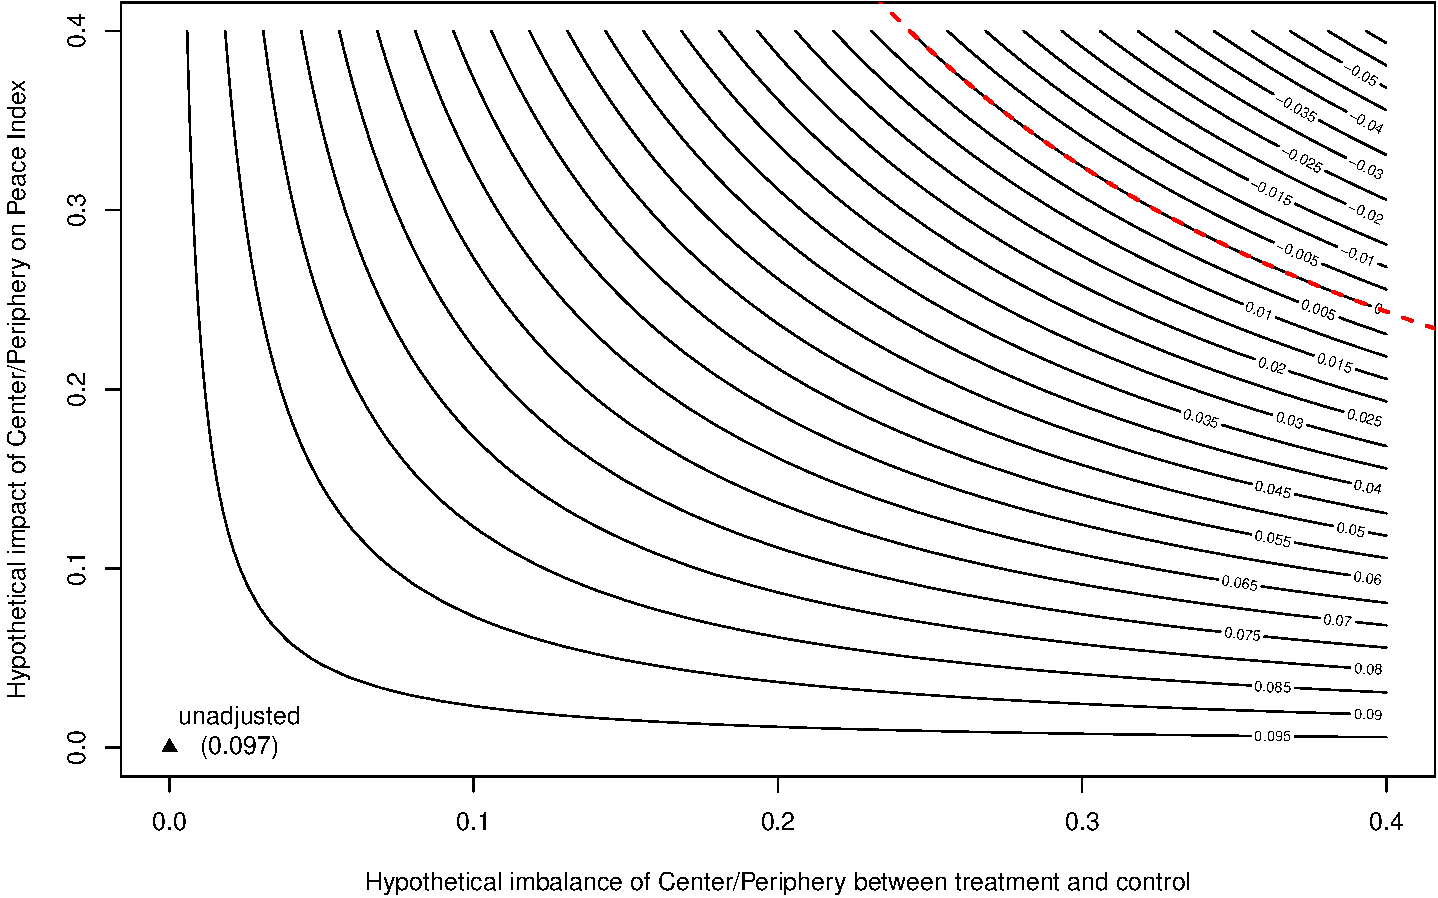
\includegraphics[width=.55\textwidth]{natural_plot_new.pdf}
\end{figure}
% \vspace{-.1in}
% \onslide<4-> Works in principle, but poor parameterization...
\end{frame}


%======================================================================
\section{$R^2$ reparameterization}
%======================================================================

\begin{frame}{Why reparameterize}
\small
\onslide<1-> Problems with the natural parameterization:
\begin{itemize}
\item<2-> ``Impact'' and ``imbalance'' are scale-dependent. \textit{Center} happened to be binary but hard for abstract confounders (e.g.\ ``political attitudes'').
\item<3-> ``Name a possible confounder'' is too narrow. We want to handle multiple confounders, possibly acting non-linearly.
\end{itemize}
\medskip
\onslide<4-> \textbf{Fix:} reparameterize using \textit{partial $R^2$}.
\begin{itemize}
\item<5-> Scale-free, intuitive, bounded in $[0,1]$
\item<6-> With this we will derive bias \textit{and} variance, do bounds, handle all confounders jointly, and more.
\end{itemize}
\end{frame}


\begin{frame}{What is the partial $R^2$?}
\small
\onslide<1-> The partial correlation is simply correlation \textit{after} partialling out $\X$:
\[
R_{Y \sim D \mid \X} \;=\; \cor(Y^{\perp \X},\, D^{\perp \X}).
\]
Square it for the partial~$R^2$.\\

\medskip
\onslide<2-> Or: ``fraction of $D$'s explained by $Z$ beyond what $\X$ explained'':   
\[
R^2_{D\sim Z \mid \X} \;=\; \frac{R^2_{D\sim \X + Z} - R^2_{D\sim \X}}{1 - R^2_{D\sim \X}}.
\]
\onslide<3-> And:
\[
R^2_{Y\sim Z \mid D, \X} \;=\; \frac{R^2_{Y\sim D + \X + Z} - R^2_{Y\sim D + \X}}{1 - R^2_{Y\sim D + \X}}.
\]
\onslide<4-> Direction-symmetric: $R^2_{D\sim Z \mid \X} = R^2_{Z \sim D \mid \X}$ 
\end{frame}


\begin{frame}{Deriving bias in the $R^2$ parameterization}
\footnotesize
\onslide<1-> By FWL,
\begin{align*}
\widehat{\bias} &= \hat{\gamma}\hat{\delta} \\
&= \left(\frac{\cov(Y^{\perp \X, D},\, Z^{\perp \X, D})}{\var(Z^{\perp \X, D})}\right) \left(\frac{\cov(D^{\perp \X},\, Z^{\perp \X})}{\var(D^{\perp \X})}\right) \\
&= \cor(Y^{\perp \X,D},\, Z^{\perp \X,D})\,\cdot\, \cor(D^{\perp \X},\, Z^{\perp \X}) \\[-2pt]
&\qquad\cdot\;  \frac{\sd(Y^{\perp \X,D})}{\sd(D^{\perp \X})} \,\cdot\,  \frac{\sd(Z^{\perp \X})}{\sd(Z^{\perp \X,D})}.
\end{align*}

\onslide<2-> Recognise:
\begin{itemize}
\item $\cor(Y^{\perp \X,D},\, Z^{\perp \X,D})^2 = R^2_{Y\sim Z \mid D, \X}$
\item $\cor(D^{\perp \X},\, Z^{\perp \X})^2 = R^2_{D\sim Z \mid \X}$
\item $\dfrac{\var(Z^{\perp \X,D})}{\var(Z^{\perp \X})} = 1 - R^2_{D\sim Z \mid \X}$
\end{itemize}

\onslide<3->
\normalsize
\[
\boxed{\;|\widehat{\bias}| \;=\; \sqrt{\frac{R^2_{Y\sim Z \mid D, \X}\, R^2_{D\sim Z \mid \X}}{1 - R^2_{D\sim Z \mid \X}}}\;
\cdot\; \frac{\sd(Y^{\perp \X, D})}{\sd(D^{\perp \X})}.\;}
\]
\end{frame}


\begin{frame}{Bias anatomy}
\small
\onslide<1-> An OLS variance fact (for now and later):
\[
\widehat{\se}(\hat{\tau}_{\text{res}}) \;=\; \frac{\sd(Y^{\perp \X, D})}{\sd(D^{\perp \X})\,\sqrt{\df}}.
\]
\onslide<2-> Nice to rewrite bias then as:
\[
|\widehat{\bias}| \;=\; \sqrt{\tfrac{R^2_{Y\sim Z \mid D,\X}\, R^2_{D\sim Z \mid \X}}{1 - R^2_{D\sim Z \mid \X}}}\cdot \frac{\sd(Y^{\perp \X, D})}{\sd(D^{\perp \X})}
\;=\; \widehat{\se}(\hat{\tau}_{\text{res}}) \cdot \sqrt{\underbrace{\tfrac{R^2_{Y\sim Z \mid D,\X}\, R^2_{D\sim Z \mid \X}}{1 - R^2_{D\sim Z \mid \X}}}_{\text{BF}^2} \cdot \df}.
\]
\onslide<3-> Consider the ``relative bias'', i.e.\ the proportion of $\hat{\tau}_{res}$ that is bias.  Substitute $|\hat{\tau}_{\text{res}}| = |t_D|\cdot \widehat{\se}(\hat{\tau}_{\text{res}})$ in the denominator ($|t_D|$ = absolute t-stat for $D$):

\[ \frac{|\widehat{\bias}|}{|\hat{\tau}_{\text{res}}|} \;=\; \frac{\widehat{\se}(\hat{\tau}_{\text{res}})\cdot \sqrt{\text{BF}^2\cdot \df}}{|t_D|\cdot \widehat{\se}(\hat{\tau}_{\text{res}})} \;=\; \frac{\sqrt{\df}\cdot \text{BF}}{|t_D|}. \]
\end{frame}

\begin{frame}{Bias anatomy:}
One last touch: 

\[ \frac{\sqrt{\df}\cdot \text{BF}}{|t_D|} = \frac{BF}{| f_{Y\sim D|\X}|} \]

\noindent where $f_{Y\sim D|\X} = R_{Y\sim D | \X}/\sqrt{1-R_{Y\sim D | \X}}$ is the (partial) Cohen's $f$.\\
\bigskip

% Cohen's $f^2$ is an ``odds ratio'' version of the $R^2$:

% \[
% f^2_{Y\sim D|\X} := \frac{R^2_{Y\sim D|\X}}{1 - R^2_{Y\sim D|\X}}
% \]
% which is a rescaling of $t_D$:
% \[
% |f_{Y\sim D|\X}| := \frac{|t_D|}{\sqrt{\df}}
% \]

% \medskip
% \onslide<2-> So we can rewrite relative bias as:
% \[
% \frac{|\widehat{\bias}|}{|\hat{\tau}_{\text{res}}|} = \frac{\text{BF}}{|f_{Y\sim D|\X}|}.
% \]
\onslide<3->  Key insights \\
\small
\begin{itemize}
\item Numerator:  BF = essential expression of confounding strength.  
\item Denominator: $f_{Y\sim D|\X}$ is essentially how much $Y$ is explained uniquely by $D$ and is \textit{all} you need from the data to understand sensitivity.  It is what confounding is competing to explain.
\item  And $f_{Y\sim D|\X}$ is not function of sample size: more data doesn't help you fight confounding.
\end{itemize}
\end{frame}


\begin{frame}{Variance anatomy}
\small
\onslide<1-> Same OLS variance fact, applied to the \textit{full} regression:
\[
\widehat{\se}(\hat{\tau}) \;=\; \frac{\sd(Y^{\perp \X, D, Z})}{\sd(D^{\perp \X, Z})\,\sqrt{\df - 1}}.
\]
\onslide<2-> Two ratios of variances are partial $R^2$'s:
\[
\frac{\sd^2(Y^{\perp \X, D, Z})}{\sd^2(Y^{\perp \X, D})} = 1 - R^2_{Y\sim Z \mid \X, D}, \quad
\frac{\sd^2(D^{\perp \X, Z})}{\sd^2(D^{\perp \X})} = 1 - R^2_{D\sim Z \mid \X}.
\]
\onslide<3-> Combine, factoring out $\widehat{\se}(\hat{\tau}_{\text{res}})$:
\[
\widehat{\se}(\hat{\tau}) \;=\; \widehat{\se}(\hat{\tau}_{\text{res}}) \cdot \sqrt{\underbrace{(1-R^2_{Y\sim Z \mid \X, D})}_{\text{VRF}}\,\underbrace{\tfrac{1}{1-R^2_{D\sim Z \mid \X}}}_{\text{VIF}}\,\underbrace{\tfrac{\df}{\df-1}}_{\text{df adj.}}}.
\]
\onslide<4->
\begin{itemize}
\item \textbf{VRF}: confounder shrinks residual $Y$ variance.
\item \textbf{VIF}: confounder's correlation with $D$ inflates the SE.
%\item \textbf{df adj.}: extra parameter in the full regression costs one df.
\end{itemize}
\end{frame}


%======================================================================
\section{Tools}
%======================================================================

\begin{frame}{Two simple statistics for routine reporting}
\small
\onslide<1-> \textbf{Robustness Value} (RV): the level of (equal) association with $D$ and $Y$ that would eliminate the effect.
\begin{itemize}
\item<2-> $\rv_{q}$: the equal-association level needed to bring the estimate down by proportion $q$
\item<3-> $\rv_{\alpha}$: the equal-association level needed to bring the t-stat to the threshold for level $\alpha$
\end{itemize}
\medskip
\onslide<4-> \textbf{Partial $R^2$ of $D$ with $Y$}: $R^2_{Y\sim D \mid \X}$
\begin{itemize}
\item<5-> If confounding explained \textit{all} residual $Y$-variance, this is how much it would have to explain of $D$ (residual variance) to bring the estimate to zero.
\end{itemize}
\medskip
\onslide<6-> Both come from $t_D$ and $\df$ alone --- you can compute them from a published regression table.
\end{frame}


\begin{frame}{Augmented regression table: Darfur}
\footnotesize
\begin{table}[!h] \centering
\begin{tabular}{lrrrrrr}
\multicolumn{7}{c}{Outcome: \textit{Peace Index}} \\
\hline\hline
Treatment: & Est. & SE & t & $R^2_{Y\sim D|\X}$ & RV & $\rv_{\alpha=0.05}$ \\
\hline
\textit{Directly Harmed} & 0.097 & 0.023 & 4.18 & 2.2\% & 13.9\% & 7.6\% \\
\hline
$\df = 783$ & & \multicolumn{5}{r}{\small \textit{Bound (1$\times$ female):}\ $R^2_y = 12\%$,\ $R^2_d = 1\%$}
\end{tabular}
\end{table}

\onslide<2->
\medskip
Cold-call check:
\begin{itemize}
\item What does this RV mean?
\item What does $\rv_{\alpha=0.05}$ mean?
\item What does $R^2_{Y\sim D \mid \X}$ mean?
\end{itemize}
\end{frame}


% \begin{frame}{Informal benchmarking is broken}
% \footnotesize
% \onslide<1-> A common move: ``a confounder \textit{not unlike} an observed $X_j$ would do this much.'' \textbf{This is biased.}
% \medskip
% \onslide<2-> When $Z$ is omitted, $\hat{\beta}_{X,\text{res}} - \hat{\beta}_X = \hat{\gamma}\hat{\psi}$, and $\hat{\psi}$ can be non-zero \textit{even if $\X \perp Z$}, because $D$ is a collider once conditioned on.
% \medskip
% \onslide<3-> Tiny DGP: $X = \epsilon_x$, $Z = \epsilon_z$, $D = X+Z+\epsilon_d$, $Y = X+Z+\epsilon_y$. No effect of $D$. $Z$ \textit{exactly} like $X$. Honest benchmarking should say ``a confounder like $X$ zeroes the effect.''
% \smallskip
% \onslide<4->
% \begin{figure}
% \centering
% 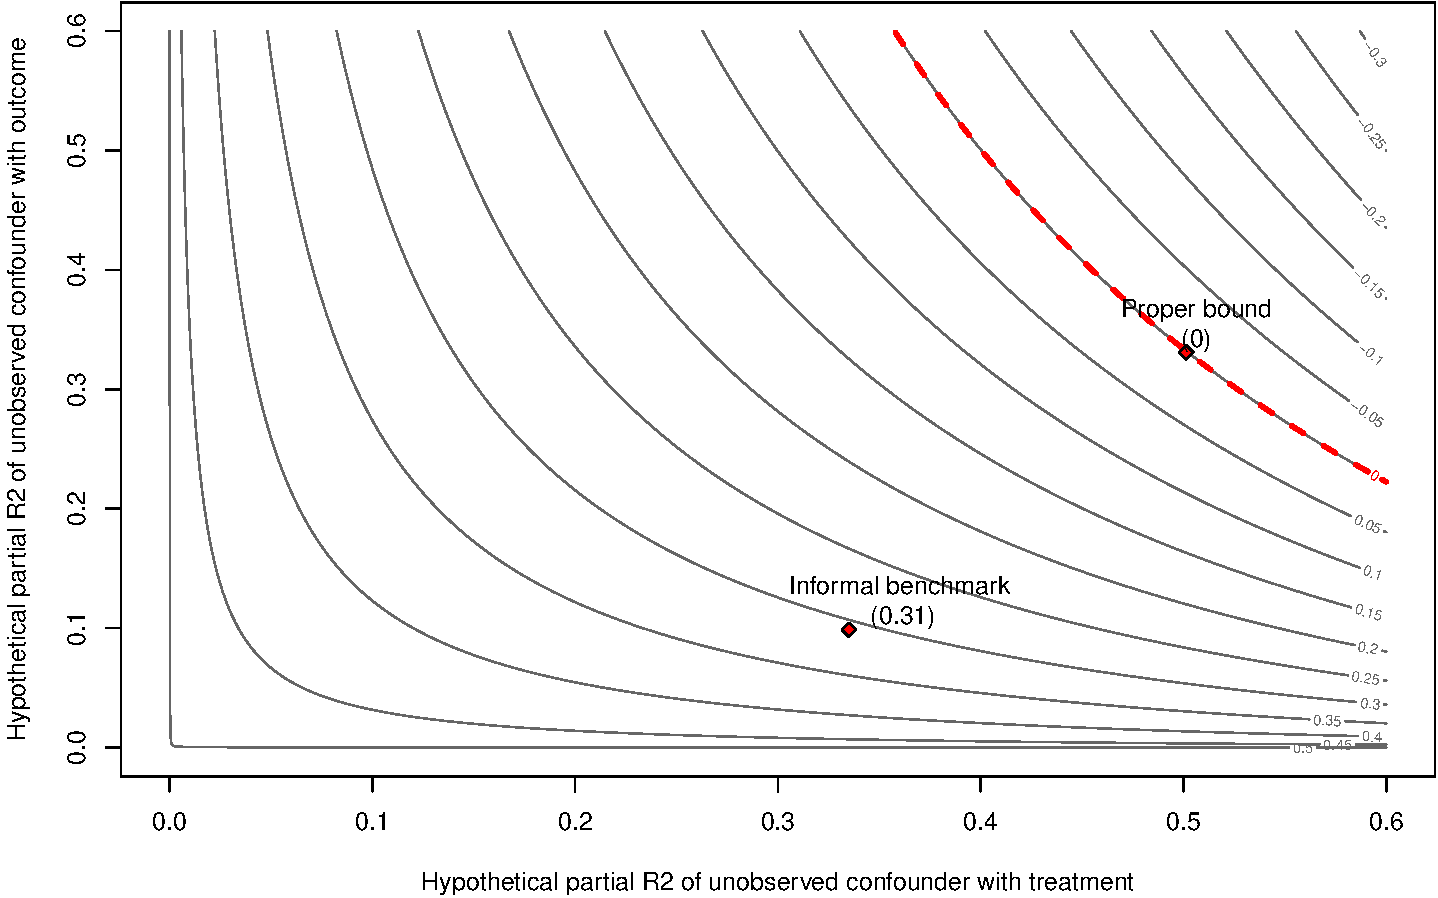
\includegraphics[width=.50\textwidth]{informal_vs_bound.pdf}
% \end{figure}
% \vspace{-.05in}
% \scriptsize Informal benchmarking (red) understates the confounding; the proper bound (blue) gets it right.
% \end{frame}


\begin{frame}{Bounding by comparison to observed covariates}
\small
\onslide<1-> ``Benchmarking'' interpretation: For an observed covariate $X_j$, define \\
\[
k_D := \frac{R^2_{D\sim Z \mid \X_{-j}}}{R^2_{D\sim X_j \mid \X_{-j}}}, \qquad
k_Y := \frac{R^2_{Y\sim Z \mid \X_{-j}, D}}{R^2_{Y\sim X_j \mid \X_{-j}, D}}.
\]
``$Z$ is at most $k_D$ times as predictive of $D$, $k_Y$ times as predictive of $Y$, as $X_j$ is.''
\medskip
\onslide<2-> Given $\{X_j, k_D, k_Y\}$, this \textit{bounds} both $R^2_{Y\sim Z|\X,D}$ and $R^2_{D\sim Z|\X}$\footnote{This is more complicated than it sounds: the observed $R^2$ of observed $X$ are themselves biased, including by collider bias from the inclusion of $D$.  But you can construct bounds; see Cinelli \& Hazlett 2020.} \\
\medskip
\onslide<3-> Yields a worst-case bias and so a worst-case adjusted estimate. Conservative for multiple, non-linear confounders.\\
\medskip
\onslide<4-> \textbf{This shows the implications of an assumption --- you have to argue the assumption itself is believable.}\\
\end{frame}


\begin{frame}{$R^2$ contour with bounds: Darfur}
\small
Within village, it is hard to argue \textit{any} basis for targeting could matter more than $\mathit{female}$. So $X_j = \mathit{female}$, with various $k$.
\begin{figure}
\centering
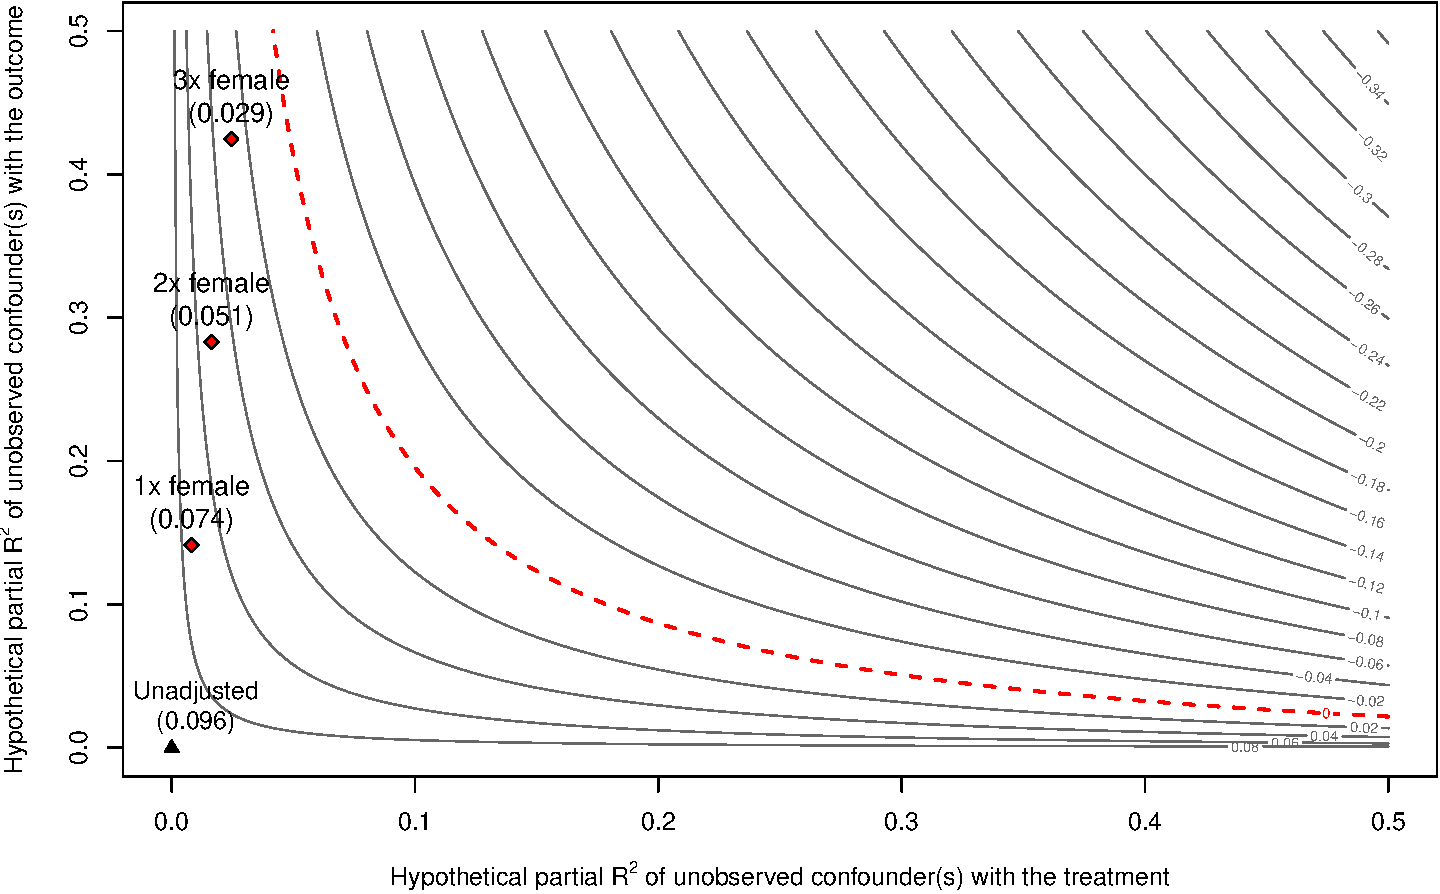
\includegraphics[scale=.45]{r2contour_female.pdf}
\end{figure}
\vspace{-.15in}
\footnotesize
Point estimate robust to a confounder $1\times$, $2\times$, even $3\times$ as strong as $\mathit{female}$.
\end{frame}


\begin{frame}{Inference and extreme scenarios}
\footnotesize
\begin{columns}[T]
\begin{column}{0.5\textwidth}
\centering
\textbf{$t$-statistic contour}\\[2pt]
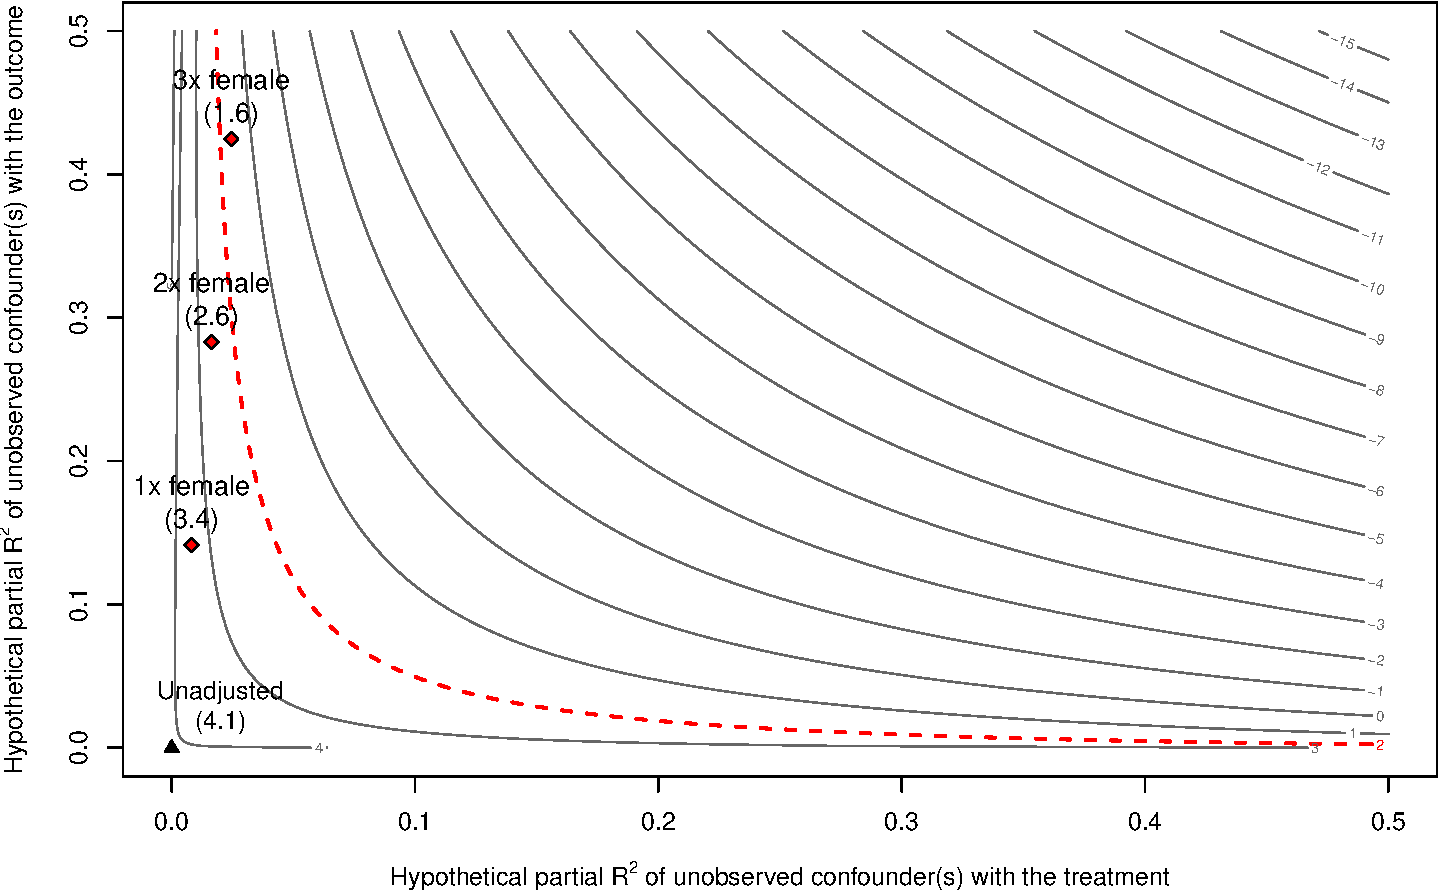
\includegraphics[width=\textwidth]{tcontour.pdf}\\[3pt]
\onslide<2->\scriptsize $t$ remains significant against a confounder up to ${\sim}2\times$ \textit{female}; loses sig.\ at $3\times$.
\end{column}
\begin{column}{0.5\textwidth}
\centering
\onslide<3-> \textbf{Extreme scenario}\\[2pt]
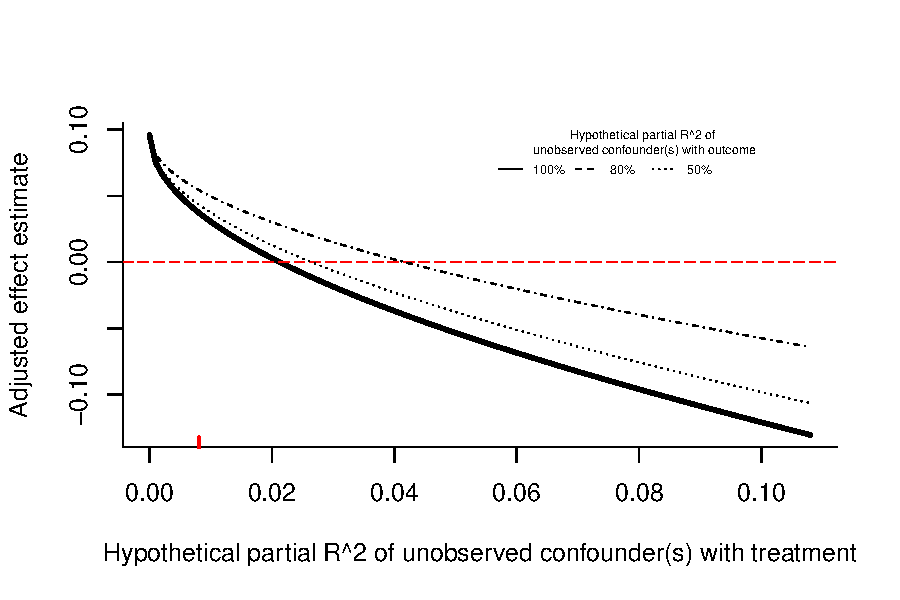
\includegraphics[width=\textwidth]{extreme_darfur.pdf}\\[3pt]
\onslide<4-> \scriptsize Assume $R^2_{Y\sim Z|\X,D} = 1$. Then $Z$ would still need to explain $\geq 2.2\%$ of $D$ to zero the effect. Pay a real price when you can't bound.
\end{column}
\end{columns}
\end{frame}


%======================================================================
\section{Practice}
%======================================================================

\begin{frame}{How to argue it, and what readers should demand}
\small
\onslide<1-> Occasionally you might be able to argue in support of a claim, e.g. in Darfur:
\scriptsize
\begin{quote}
``\dots aircraft dropped makeshift and unguided bombs over villages, and militia raided without concern for who they would attack --- the only known major exception, due to sexual assaults, was targeting gender, which is also one of the most visually apparent characteristics. \textbf{A confounder twice as strong as \textit{female} would be surprising.}''
\end{quote}
\bigskip
\small
\onslide<2-> Flipside: dismissing a result requires arguing for confounding of a given strength. (And all you need is $t$ and $df$ to get started)\\
% \begin{itemize}
%   \footnotesize
% \item Not that as a reader or reviewer: $t$ and $\df$ alone let \textit{you} compute the RV --- no excuse not to.
% \end{itemize}
\bigskip
\onslide<3-> More broadly, remember:
\footnotesize
\begin{itemize}
  \item No magic RV threshold:  refine the debate, not hide behind a number.
  \item This is never ``how much feasible confounding is there'' --- it's ``how much confounding would it take to overturn the conclusion''
  \item The result might be informative or might show that we can't say much, but either way it is the honest conversation.
\end{itemize}
% \begin{itemize}
% \item Report RV, $\rv_{\alpha=0.05}$, and $R^2_{Y\sim D \mid \X}$
% \item Defend (or refuse to defend) bounds via observed covariates
% \item Show extreme-scenario plot if you can't defend bounds
% \item As a reader: $t$ and $\df$ alone let \textit{you} compute the RV --- no excuse not to
% \item Remember: ..
% \end{itemize}
%\medskip
\end{frame}


% \begin{frame}{Beyond CI: sensitivity for other ID strategies}
% \small
% \onslide<1-> This won't make sense yet but will when you come back.\\
% \medskip
% \onslide<2-> Sensitivity tools exist for many ID strategies. The trick is choosing a useful violation to parameterize, e.g.\\
% \begin{itemize}
% \item<2-> \textbf{IV}: See extra slides below. Violations of exclusion + ignorability of the instrument; same OVB machinery.
% \item<3-> \textbf{DID:} consider non-parallelness of trends (maybe as multiples of pre-trend differences ) or consider a pre-treatment outcome to be a placebo with possibly different strength of confounding. Could use OLS OVB with difference score as well.
% %\item<4-> \textbf{Mediation, panels, weighting:} active areas of development.
% \end{itemize}
% \bigskip
% \onslide<5-> \textbf{The bigger picture:} move from ``is it identified?'' to ``how much would assumptions have to fail to overturn the conclusion?''
% \medskip
% \onslide<6-> Software: \texttt{sensemakr} (R, Stata) --- \href{http://carloscinelli.com/sensemakr/}{carloscinelli.com/sensemakr}.
% \end{frame}


\begin{frame}{Resources}
\small
\textbf{Papers} (all linked from \href{https://chadhazlett.com/publications.html}{chadhazlett.com/publications}):
\begin{itemize}
\item Cinelli \& Hazlett (2020). \textit{Making sense of sensitivity: Extending omitted variable bias.} JRSS B. --- the framework
\item Hazlett \& Parente (2023). \textit{From ``Is it unconfounded?'' to ``How much confounding would it take?''} JoP. --- applied / how-to-argue companion
\item Cinelli, Ferwerda \& Hazlett (2024). \textit{sensemakr: Sensitivity Analysis Tools for OLS in R and Stata.} Observational Studies. --- software paper
\item Cinelli \& Hazlett (2025). \textit{An OVB framework for sensitivity analysis of IV.} Biometrika. --- IV extension (cf.\ extras)
\end{itemize}
\medskip
\textbf{Software \& tutorials}:
\begin{itemize}
\item \texttt{sensemakr} R/Stata + worked vignettes: \href{http://carloscinelli.com/sensemakr/}{carloscinelli.com/sensemakr}
\item Carlos Cinelli's site (talks, tutorials, videos): \href{http://carloscinelli.com}{carloscinelli.com}
\item Software list on my site: \href{https://chadhazlett.com/software.html}{chadhazlett.com/software}
\end{itemize}
\end{frame}


%======================================================================
\appendix
%======================================================================

\section{Extra slides: matched-pair $\Gamma$ bounds}

\begin{frame}{Rosenbaum's $\Gamma$ for matched pairs}
\small
\begin{itemize}
\item<1-> A different sensitivity tradition (Rosenbaum 2002), with a single parameter $\Gamma \geq 1$ quantifying departure from zero confounding.
\smallskip
\item<2-> Consider matched pairs $i$ and $j$ with $X_i = X_j$. Under SOO, both have the same $\pi(X)$.
\smallskip
\item<3-> A binary unobserved $U$ may make their odds of treatment differ:
\[
\frac{1}{\Gamma} \;\leq\; \frac{\pi_i(1-\pi_j)}{(1-\pi_i)\pi_j} \;\leq\; \Gamma.
\]
\end{itemize}
\end{frame}


\begin{frame}{Formal sensitivity tests ($\Gamma$)}
\small
\begin{itemize}
\item<1-> $\Gamma = 1$: no hidden bias. $\Gamma = 2$: unit $i$ has twice the odds of treatment as $j$ despite identical $X$.
\smallskip
\item<2-> ``Primal'' version: only the odds of \textit{treatment} are varied; effect of $U$ on the outcome is taken to be infinite (worst-case).
\smallskip
\item<3-> At any chosen $\Gamma$, run a permutation-style test where assignment odds respect $\Gamma$.
\smallskip
\item<4-> Try increasing $\Gamma$ until significance is lost or the sign flips.
\smallskip
\item<5-> R: \texttt{psens()}, \texttt{hlsens()} in \texttt{rbounds}.
\end{itemize}
\end{frame}


\begin{frame}{Rosenbaum-style sensitivity: smoking example}
\small
\begin{figure}
\centering
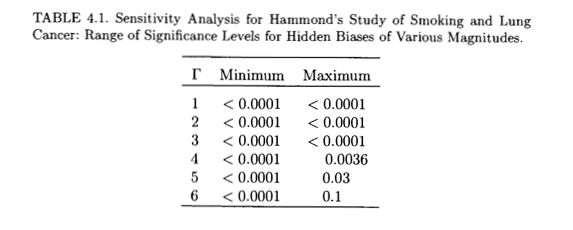
\includegraphics[scale=.5]{smoking_sensitivity.png}
\end{figure}
\onslide<2-> If a hidden confounder gave the unit with the worse outcome 6$\times$ higher odds of smoking, the adjusted estimate would lose significance.
\end{frame}


\section{Extra slides: parametric (Imbens 2003)}

\begin{frame}{Imbens (2003): parametric approach}
\footnotesize
\begin{itemize}
\item Highly parametric:
\begin{itemize}\smallskip
\item Assume $Y_1, Y_0 \indep D \mid X, U$ with $U \sim \mathrm{Bernoulli}(0.5)$, $U \perp X$.\smallskip
\item Logistic propensity: $P(D=1 \mid X, U) = \dfrac{\exp(X\theta + \gamma U)}{1 + \exp(X\theta + \gamma U)}$. Here $\gamma$ governs $U$--$D$ strength.\smallskip
\item Outcome conditionally normal: $Y \mid X, U \sim N(\alpha D + X\beta + \delta U,\ \sigma^2)$. $\delta$ governs $U$--$Y$ strength.\smallskip
\item Choose $(\gamma, \delta)$, MLE for $\hat{\alpha}(\gamma, \delta)$.
\end{itemize}
\item Reparameterize $(\gamma, \delta)$ as partial $R^2$'s with $D$ and with $Y$ for interpretability.
\end{itemize}
\bigskip
Trades stronger assumptions for more direct probabilistic interpretation. Carnegie--Dorie--Hill (2016) extends with BART for $\mu_0(X)$.
\end{frame}


\section{Extra slides: IV-OVB sensitivity}

\begin{frame}{OVB with instrumental variables}
\small
We can apply the same OVB machinery to IV. Walks through, applied to the Card (1993) returns-to-education example.
\end{frame}


\begin{frame}{Running example: returns to education (Card 1993)}
\small
\begin{itemize}
\item<1-> Estimating returns to education has long been a challenge.
\item<2-> OLS with $N=3010$, covariates $X = \{$race, experience, regional$\}$ suggests 7.5\% higher earnings per year of education.
\item<3-> Confounding may be severe: ability, motivation, family/social.
\item<4-> Card uses \textit{proximity to college} as instrument.
\end{itemize}
\end{frame}


\begin{frame}{These assumptions may fail!}
\small
The IV estimate can be biased --- worse than OLS --- if \textit{Proximity} is not a valid instrument due to uncontrolled:
\smallskip
\begin{itemize}
\item<2-> ``side-effects'' (e.g.\ high-wage jobs near colleges)
\item<3-> ``common-cause confounders'' (e.g.\ unmeasured SES)
\end{itemize}
\onslide<4->
\smallskip
\vspace{-.1in}
\begin{figure}[!ht]
\centering
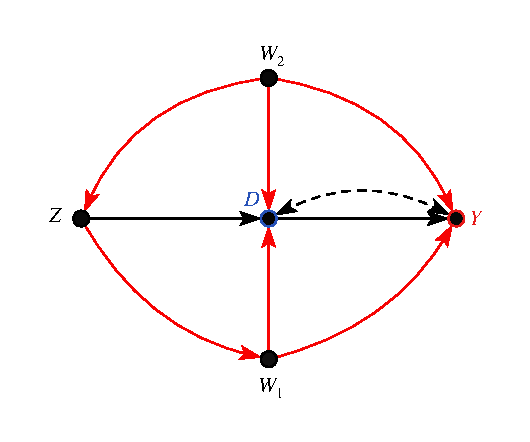
\includegraphics[scale=0.6]{figures/IV_violations_solid.pdf}
\label{fig:bogusIV}
\end{figure}
\vspace{-.3in}
\medskip
\onslide<5->
\begin{center}
\textcolor{blue}{How ``bad'' would such violations need to be to change the conclusion?}
\end{center}
\end{frame}


\begin{frame}{IV regression: three estimators}
\onslide<1-> \textbf{1. Indirect least squares:}
\onslide<2-> \begin{align*}
\text{Reduced form:} & \quad \text{Earnings} = \hat{\lambda}_{\text{res}}\,\text{Proximity} + \X\hat{\beta}_{\text{res}} + \hat{\epsilon}_{y, \text{res}} \\
\text{First stage:} & \quad \text{Education} = \hat{\theta}_{\text{res}}\,\text{Proximity} + \X\hat{\psi}_{\text{res}} + \hat{\epsilon}_{d, \text{res}}
\end{align*}
\bigskip

\onslide<3-> \textbf{2. Two-stage least squares:}
\begin{align*}
\text{2nd stage:} & \quad \text{Earnings} = \hat{\tau}_{\text{2SLS}, \text{res}}\,\widehat{\text{Education}} + \X\hat{\beta}_{\text{2SLS},\text{res}} + \hat{\epsilon}_{\text{2SLS}, \text{res}}
\end{align*}

\onslide<4-> Same answer:
\vspace{-.2in}
\begin{align*}
\hat{\tau}_{\text{2SLS}} = \hat{\tau}_{\text{ILS}} := \frac{\hat{\lambda}_{\text{res}}}{\hat{\theta}_{\text{res}}} = \frac{0.042}{0.319} \approx 0.132.
\end{align*}
\end{frame}


\begin{frame}{IV regression: Anderson--Rubin}
\textbf{3. Anderson--Rubin (Fieller):}
\begin{align*}
\text{Earnings} - \tau_0 \text{Education} = \hat{\phi}_{\tau_0,\text{res}}\,\text{Proximity} + \X\hat{\beta}_{\tau_0,\text{res}} + \hat{\epsilon}_{\tau_0, \text{res}}
\end{align*}
\small
\begin{itemize}
\item $\tau_0$ that makes $\hat{\phi}_{\tau_0,\text{res}} = 0$ is the point estimate
\item $\{\tau_0 : \text{do not reject } \hat{\phi}_{\tau_0,\text{res}} = 0\}$ is the CI
\item Correct coverage regardless of instrument strength
\end{itemize}
\bigskip
\onslide<2-> All give 13.2\% higher earnings per year of education.
\medskip
\begin{center}
\onslide<3-> \textcolor{blue}{How would these change had we included $W$?}
\end{center}
\end{frame}


\begin{frame}{Start with the reduced form}
\onslide<1-> We wanted to run
\begin{align*}
Y = \hat{\lambda}\, Z + \X\hat{\beta} + \hat{\gamma} W + \hat{\epsilon}_y.
\end{align*}
\medskip
\onslide<2-> But $W$ was not observed, so we ran
\begin{align*}
Y = \hat{\lambda}_{\text{res}}\, Z + \X\hat{\beta}_{\text{res}} + \hat{\epsilon}_{y,\text{res}}.
\end{align*}
\medskip
\onslide<3-> \textcolor{blue}{How would including $W$ change inference about $\lambda$?}
\end{frame}


\begin{frame}{Same OVB analysis, different variable names}
\begin{itemize}
\item $R^2_{Y\sim W \mid Z, \X}$: $W$'s share of outcome variance
\item $R^2_{Z\sim W \mid \X}$: $W$'s share of \textit{instrument} variance
\end{itemize}
\onslide<2->
\begin{align*}
|\widehat{\bias}|
&= \sqrt{\frac{R^2_{Y\sim W \mid Z, \X}\, R^2_{Z\sim W \mid \X}}{1 - R^2_{Z\sim W \mid \X}}\,\df}\,\cdot\,\widehat{\se}(\hat{\lambda}_{\text{res}}) \\
&= \BF\sqrt{\df}\,\cdot\,\widehat{\se}(\hat{\lambda}_{\text{res}})
\end{align*}
\onslide<3->
\begin{align*}
\widehat{\se}(\hat{\lambda})
&= \sqrt{\frac{1 - R^2_{Y\sim W \mid Z, \X}}{1 - R^2_{Z\sim W \mid \X}}\,\frac{\df}{\df-1}}\,\cdot\,\widehat{\se}(\hat{\lambda}_{\text{res}}) \\
&= \SeF\sqrt{\df/(\df-1)}\,\cdot\,\widehat{\se}(\hat{\lambda}_{\text{res}})
\end{align*}
\end{frame}


\begin{frame}{An embarrassingly simple sensitivity analysis}
\begin{center}
\textit{Change the critical $t$ rather than the point estimate.}
\end{center}
\medskip

\onslide<2-> Familiar $1-\alpha$ CI:
\begin{align*}
\hat{\lambda}_{\text{res}} \pm t^*_{\alpha, \df} \cdot \widehat{\se}(\hat{\lambda}_{\text{res}}).
\end{align*}

\onslide<3-> Adjust for confounding (limited by $\R^2$):
\begin{align*}
\hat{\lambda}_{\text{res}} \pm \textcolor{blue}{t^\dagger_{\alpha, \df-1, \R^2}} \cdot \widehat{\se}(\hat{\lambda}_{\text{res}}),
\end{align*}

\onslide<4-> where
\begin{align*}
t^\dagger_{\alpha, \df-1, \R^2} := \SeF\sqrt{\df/(\df-1)} \cdot t^*_{\alpha, \df-1} + \BF\sqrt{\df}.
\end{align*}
\end{frame}


\begin{frame}{Routine reporting: (extreme) robustness values}
What would it take to reduce the coefficient until we no longer reject (with confidence $1-\alpha$) that it is $100q\%$ as large?
\bigskip

\onslide<2-> Using the RF coefficient:
\begin{itemize}
\item $\rv_{q,\alpha}(\lambda)$: minimal strength of association with both $Z$ and $Y$ needed.
\medskip
\item $\xrv_{q,\alpha}(\lambda)$: minimal strength with $Z$ alone, even if $W$ explains \textit{all} residual outcome variance.
\end{itemize}
\end{frame}


\begin{frame}{Sensitivity of RF and FS}
\small
\onslide<1-> What can we learn about IV from sensitivity of RF and FS?
\medskip
\onslide<2-> Recall ${\tau} = {\lambda}/{\theta}$.

\onslide<3-> \textbf{Sensitivity of reduced form:} for $H_0: \tau = 0$, sensitivity of RF \textit{is exactly} sensitivity of IV.
\begin{center}
\textit{``If it ain't in the reduced form, it ain't there.''} (Angrist \& Pischke)
\end{center}

\onslide<4-> \textbf{Sensitivity of first stage:} If the sign of the FS isn't guaranteed, you cannot rule out unbounded estimates / CIs.

\onslide<5-> AR is consistent with this logic.
\end{frame}


\begin{frame}{Sensitivity with the AR regression}
\small
\[
Y_{\tau_0} = \hat{\phi}_{\tau_0, \text{res}}\, Z + \X\hat{\beta}_{\tau_0, \text{res}} + \hat{\epsilon}_{\tau_0, \text{res}}
\]

The AR confidence interval:
\begin{align*}
\text{CI}_{1-\alpha}(\tau) = \left\{\tau_0 :\; t^2_{\hat{\phi}_{\text{res}, \tau_0}} \leq (t^*_{\alpha, \df-1})^2\right\}.
\end{align*}

Replace $t^*_{\alpha, \df-1}$ with $t^{\dagger\,\max}_{\alpha, \df-1, \R^2}$:
\begin{align*}
\text{CI}^{\max}_{1-\alpha, \R^2}(\tau) = \left\{\tau_0 :\; t^2_{\hat{\phi}_{\text{res}, \tau_0}} \leq (t^{\dagger\,\max}_{\alpha, \df-1, \R^2})^2\right\}.
\end{align*}
\footnotesize
Analytical solution via quadratic inequality. Yields $\rv_{q,\alpha}(\tau)$, $\xrv_{q,\alpha}(\tau)$ and $\rv_{\geq q,\alpha}(\tau)$, $\xrv_{\geq q,\alpha}(\tau)$.
\end{frame}


\begin{frame}{Card example: sensitivity of RF and FS}
\onslide<2-> \textbf{1. Reduced form: $H: \tau = 0$.}
\footnotesize
\begin{table}[!ht]
\centering
\begin{tabular}{lrrrrrr}
\multicolumn{7}{c}{Outcome: \textit{Earnings} (log)} \\
\hline\hline
Instrument & Est. & SE & t & $R^2_{Y\sim Z \mid \X}$ & $\xrv_{q^*,\alpha}$ & $\rv_{q^*,\alpha}$ \\
\hline
\textit{Proximity} & 0.042 & 0.018 & 2.33 & 0.18\% & 0.05\% & 0.67\% \\
\hline
\multicolumn{7}{l}{\small \textit{Bound (1$\times$ smsa):}\ $R^2_{Y\sim W|Z,\X} = 2\%$,\ $R^2_{Z\sim W|\X} = 0.6\%$,\ $t^\dagger = 2.55$}\\
\multicolumn{7}{l}{\small $\df = 2994,\ q^* = 1,\ \alpha = 0.05$}
\end{tabular}
\end{table}
\normalsize
\bigskip
\onslide<3-> \textbf{2. First stage: stability.}
\footnotesize
\begin{table}[!b]
\centering
\begin{tabular}{lrrrrrr}
\multicolumn{7}{c}{Outcome: \textit{Education} (years)} \\
\hline\hline
Instrument & Est. & SE & t & $R^2_{D\sim Z \mid \X}$ & $\xrv_{q^*,\alpha}$ & $\rv_{q^*,\alpha}$ \\
\hline
\textit{Proximity} & 0.32 & 0.088 & 3.64 & 0.44\% & 0.31\% & 3.02\% \\
\hline
\multicolumn{7}{l}{\small \textit{Bound (1$\times$ smsa):}\ $R^2_{D\sim W|Z,\X} = 0.5\%$,\ $R^2_{Z\sim W|\X} = 0.6\%$,\ $t^\dagger = 2.26$}
\end{tabular}
\end{table}
\end{frame}


\begin{frame}{Card example: reduced form contours}
\begin{figure}[!t]
\centering
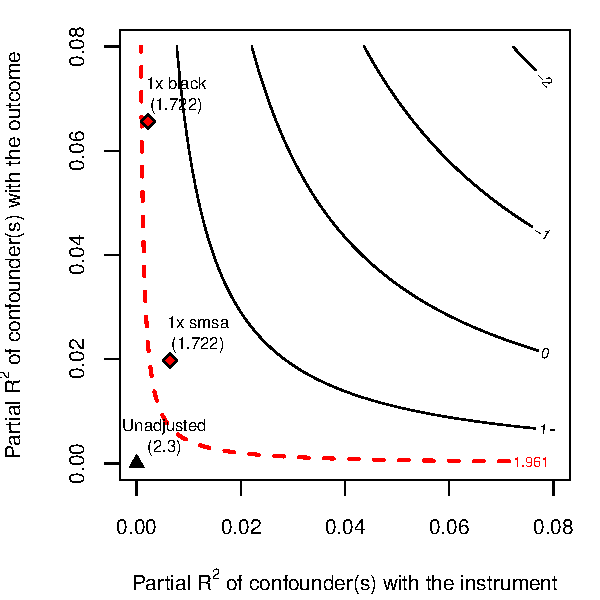
\includegraphics[scale=.75]{figures/card_reduced_form_t-value}
\caption{Sensitivity contours: reduced form}
\end{figure}
\end{frame}


\begin{frame}{Card example: sensitivity of the IV (AR)}
\begin{table}[!ht]
\centering
\begin{tabular}{lrrrrrr}
\multicolumn{7}{c}{Outcome: \textit{Earnings} (log)} \\
\hline\hline
Treatment & Est. & $\text{LL}$ & $\text{UL}$ & t & $\xrv_{\geq q^*,\alpha}$ & $\rv_{\geq q^*,\alpha}$ \\
\hline
\textit{Education} & 0.132 & 0.025 & 0.285 & 2.33 & 0.05\% & 0.67\% \\
\hline
\multicolumn{7}{l}{\small \textit{Bound (1$\times$ smsa):}\ $R^2_{Y_0\sim W|Z,\X} = 2\%$,\ $R^2_{W\sim Z|\X} = 0.6\%$,\ $t^\dagger = 2.55$}\\
\multicolumn{7}{l}{\small $\df = 2994,\ q^* = 1,\ \alpha = 0.05$}
\end{tabular}
\caption{Minimal sensitivity reporting of IV (AR)}
\end{table}

\begin{itemize}
\item<2-> Identical to RF results because the null is $\tau = 0$.
\item<3-> More interesting under other null hypotheses.
\end{itemize}
\end{frame}


\begin{frame}{Card example: CI-limit contours}
\begin{figure}[!b]
\centering
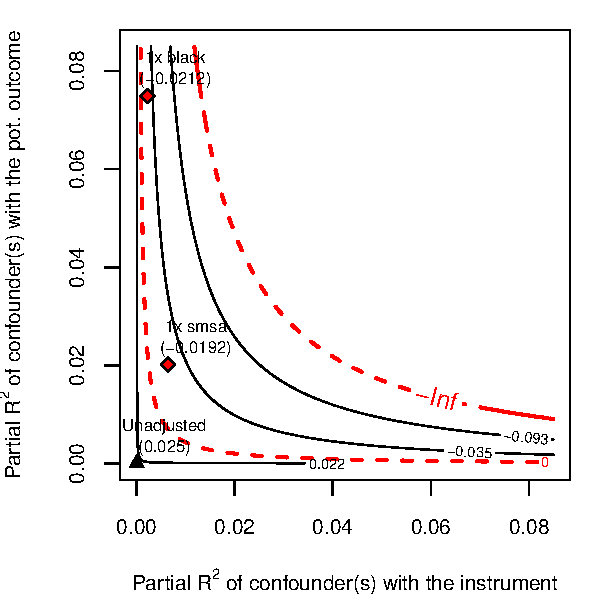
\includegraphics[scale=.6]{figures/card_iv_lower_limit}
\caption{Sensitivity contours: lower 95\% limit}
\end{figure}
\end{frame}


\begin{frame}{IV sensitivity: conclusions}
\begin{itemize}
\item OLS sensitivity to confounding can be as simple as adjusting your critical value.
\item For null of zero in IV, sensitivity of the reduced form \textit{is all you need}.
\item General sensitivity for IV is also easy: in the AR framework, explore how postulated confounding moves point estimates, CI limits, RVs, and bounds.
\end{itemize}
\end{frame}


\end{document}
